\documentclass[tikz, convert={density=300,size=1920x1080,outext=.png}]{standalone}

\pgfdeclarelayer{last}
\pgfdeclarelayer{middle-3}
\pgfdeclarelayer{middle-2}
\pgfdeclarelayer{middle-1}
\pgfdeclarelayer{second}
\pgfdeclarelayer{first}
\pgfsetlayers{last,middle-3,middle-2,middle-1,second,first,main}


% \pgfdeclarelayer{x2-m1}
% \pgfdeclarelayer{x2-m2}
% \pgfdeclarelayer{x2-m3}
% \pgfdeclarelayer{x3}
% \pgfdeclarelayer{x4}
% \pgfdeclarelayer{x1}
% \pgfsetlayers{x4,x3,x2-m1,x2-m2,x2-m3,x1,main}  % set the order of the layers (main is the standard layer)

\tikzset{
    % neurons
    neuron/.style={
        circle,
        draw=none,
        shading=ball,
        ball color=gray,
        minimum size=1cm
    },
    neuron-missingvert/.style={
        draw=none,
        scale=4,
        text height=0.3333cm,
        fill=none,
        execute at begin node=\color{black}$\vdots$
    },
    neuron-missingdiag/.style={
        draw=none,
        scale=4,
        text height=0.3333cm,
        execute at begin node=\color{black}$\ddots$
    },
    neuron-blank/.style={
        draw=none,
    },
    neuron-missing/.style={
        draw=none,
        scale=4,
        text height=0.25cm,
        execute at begin node=\color{black}$\cdotp$
    },
    % arrows
    first-layer/.style={
        line width=2pt,
        color=black!80,
        opacity=.8
    },
    second-layer/.style={
        line width=2pt,
        opacity=.4
    },
    last-layer/.style={
        line width=2pt,
        opacity=.1
    }
}

\begin{document}
    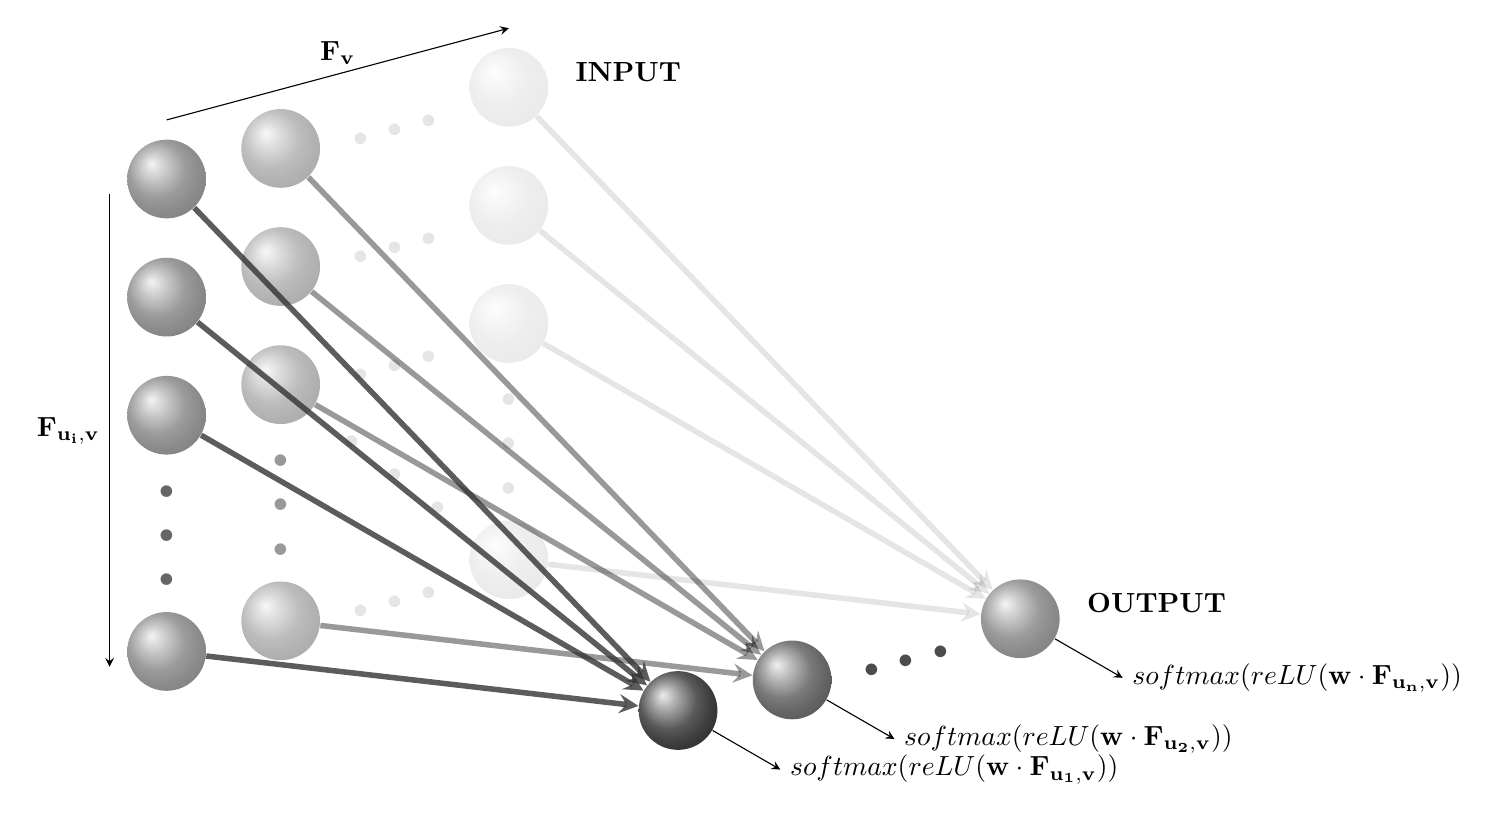
\begin{tikzpicture}[x=(15:1.5cm), y=(90:1.5cm), z=(330:1.5cm), >=stealth]

        \begin{pgfonlayer}{last}
            % draw nodes
            \foreach \m [count=\y] in {1, 2, 3, 4, 5} {
                \ifnum\m=4
                    \node [neuron-missingvert, opacity=.1] at (3, -\y, 0) {};
                \else
                    \node [neuron, opacity=.1] (input-3\m) at (3, -\y, 0) {};
                \fi
            }
            \node [neuron, opacity=.6] (output-3) at (3, -3, 5) {};

            % draw edges
            \foreach \m in {1, 2, 3, 5}
                \draw[->, last-layer] (input-3\m) -- (output-3);
        \end{pgfonlayer}

        \begin{pgfonlayer}{middle-3}
            \foreach \m [count=\y] in {1, 2, 3, 4, 5} {
                \ifnum\m=4
                    \node [neuron-blank] at (2.3, -\y, 0) {};
                \else
                    \node [neuron-missing, opacity=.1] at (2.3, -\y, 0) {};
                \fi
            }
            \node [neuron-missing, opacity=.7] at (2.3, -3, 5) {};
        \end{pgfonlayer}

        \begin{pgfonlayer}{middle-2}
            \foreach \m [count=\y] in {1, 2, 3, 4, 5} {
                \ifnum\m=4
                    \node [neuron-missingdiag, opacity=.1] at (2, -\y, 0) {};
                \else
                    \node [neuron-missing, opacity=.1] at (2, -\y, 0) {};
                \fi
            }
            \node [neuron-missing, opacity=.7] at (2, -3, 5) {};
        \end{pgfonlayer}

        \begin{pgfonlayer}{middle-1}
            \foreach \m [count=\y] in {1, 2, 3, 4, 5} {
                \ifnum\m=4
                    \node [neuron-blank] at (1.7, -\y, 0) {};
                \else
                    \node [neuron-missing, opacity=.1] at (1.7, -\y, 0) {};
                \fi
            }
            \node [neuron-missing, opacity=.7] at (1.7, -3, 5) {};
        \end{pgfonlayer}

        \begin{pgfonlayer}{second}
            % draw nodes
            \foreach \m [count=\y] in {1, 2, 3, 4, 5} {
                \ifnum\m=4
                    \node [neuron-missingvert, opacity=.4] at (1, -\y, 0) {};
                \else
                    \node [neuron, opacity=.4] (input-2\m) at (1, -\y, 0) {};
                \fi
            }
            \node [neuron, opacity=.8] (output-2) at (1, -3, 5) {};

            % draw edges
            \foreach \m in {1, 2, 3, 5}
                \draw[->, second-layer] (input-2\m) -- (output-2);
        \end{pgfonlayer}

        \begin{pgfonlayer}{first}
            % draw nodes
            \foreach \m [count=\y] in {1, 2, 3, 4, 5} {
                \ifnum\m=4
                    \node [neuron-missingvert, opacity=.6] at (0, -\y, 0) {};
                \else
                    \node [neuron, opacity=.6] (input-1\m) at (0, -\y, 0) {};
                \fi
            }
            \node [neuron] (output-1) at (0, -3, 5) {};

            % draw edges
            \foreach \m in {1, 2, 3, 5}
                \draw[->, first-layer] (input-1\m) -- (output-1);
        \end{pgfonlayer}

        % markings
        \draw [->] (-.5, -1, 0)  -- (-.5, -5, 0)   node [midway, left] {$\mathbf{F_{u_i, v}}$};
        
        \draw [->] (0, -.5, 0)  -- (3, -.5, 0)   node [midway, above] {$\mathbf{F_{v}}$};
        
        \foreach \l [count=\i] in {1, 2, n}
        \draw [->] (output-\i) -- ++(0, 0, 1) node [right] {$softmax(reLU(\mathbf{w} \cdot \mathbf{F_{u_\l, v}}))$};
       
        
        % names
        \node [align=center, right] at (3.5, -1, 0) {\textbf{INPUT}};
        \node [align=center, right] at (3.5, -3, 5) {\textbf{OUTPUT}};


        


        %    \foreach \m [count=\y] in {1, 2, 3, missing, 4} {
        %        \node [every neuron/.try, neuron \m/.try] (input-2\m) at (1, 2.5-\y, 0) {};
        %    }
        %    
        %    \foreach \i [count=\x] in {1, 2, 3, 4} {
        %        %\shade[ball color=gray!40, opacity=0.4] (\x-2.5, 0, 5) circle (0.5cm);
        %        %\draw (\x-2.5, 0, 5) circle (0.5cm) {input-\x\y};
        %        \node [every neuron] (output-\x) at (\x-2.5, 0, 5) {};
        %    }
        %\foreach \m [count=\y] in {1,2,3,missing,4}
        %\node [every neuron/.try, neuron \m/.try] (input-\m) at (0,-\y, 0) {};

        %\foreach \m [count=\y] in {1,missing,2}
        %\node [every neuron/.try, neuron \m/.try ] (hidden-\m) at (2,2-\y*1.25) {};

        %\foreach \m [count=\y] in {1,missing,2}
        %\node [every neuron/.try, neuron \m/.try ] (output-\m) at (4,1.5-\y) {};

        %\foreach \l [count=\i] in {1,2,3,n}
        %\draw [<-] (input-\i) -- ++(-1,0)
        %node [above, midway] {$I_\l$};

        %\foreach \l [count=\i] in {1,n}
        %\node [above] at (hidden-\i.north) {$H_\l$};

        %\foreach \l [count=\i] in {1,n}
        %\draw [->] (output-\i) -- ++(1,0)
        %node [above, midway] {$O_\l$};

        %\foreach \x in {1, ..., 4}
        %    \foreach \y in {1,...,4}
        %        \draw [->] (input-\x\y) -- (output-\x);

        %\foreach \i in {1,...,2}
        %\foreach \j in {1,...,2}
        %\draw [->] (hidden-\i) -- (output-\j);

        %\foreach \l [count=\x from 0] in {Input, Hidden, Ouput}
        %\node [align=center, above] at (\x*2,2) {\l \\ layer};

    \end{tikzpicture}
\end{document}
